\chapter{DevOps}
Le mouvement DevOps, contraction de « Development » et « Operational » tente de répondre à la problématique, certainement aussi ancienne que les DSI, qu’est la frontière qui sépare les développeurs (ceux qui écrivent le code source) et l’exploitation (ceux qui déploient et exploitent).\\

\begin{figure}
  \begin{center}
    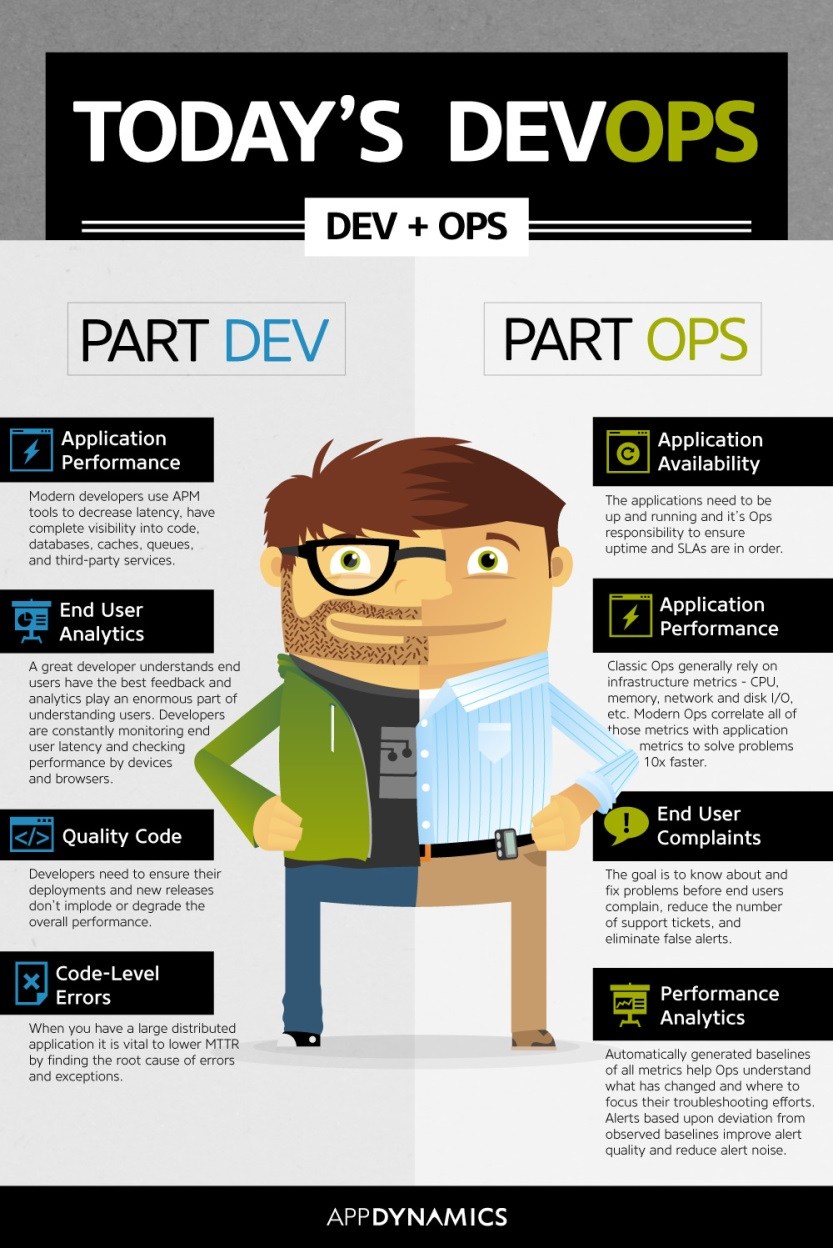
\includegraphics[scale=1.5]{images/devops.png}
  \end{center}
  \caption{DEV + OPS}
  \label{Devops}
\end{figure}

Les attentes et perspectives autour de Devops sont nombreuses :\\

\begin{itemize}
  \item \textbf{Des cycles de déploiement plus courts} : les DevOps jouent un rôle clé dans la réduction du temps du cycle de déploiement des logiciels, passant de quelques semaines à seulement quelques heures, permettant une plus grande flexibilité quant aux nouvelles fonctionnalités et changements à apporter au produit initial.
  \item \textbf{Mise à disposition de nouveaux services plus rapidement} : des déploiements fréquents associés à des délais de livraison plus rapides permettent une agilité opérationnelle.
  \item \textbf{Une satisfaction client améliorée} : grâce à des applications ciblées et de qualité, conformes aux retours clients end to end.
  \item \textbf{Des coûts réduits} : L’automatisation permet aux équipes de réaffecter des ressources précieuses à des tâches à plus haute valeur.
  \item \textbf{Conformité et Gouvernance} : Automatisation du tracking et reporting end-to-end sur les phases de livraison/déploiement contenu.\\
\end{itemize}

\section{« The Wall of Confusion »}

\section{La Culture}

\section{« Infrastructure As Code »}

http://blog.octo.com/et-si-devops-nous-emmenait-vers-tdi-test-driven-infrastructure/
